\section{Pseudoharmonic betatron oscillations}\label{sec:2.6}
We have seen that the betatron oscillations -- in either $x$ or $y$ -- are described by a pseudo-harmonic oscillation whose representative form is
\begin{align}
	x(s) &= a\sqrt{\beta}\ \cos\{\varphi-\vartheta\}\label{eq:2.46}\\
	\varphi &= \int_{0}^{s} \frac{d\bar{s}}{\beta}\label{eq:2.47}
\end{align}
where $\beta$ is a given function of $s$, which we may call the betatron function, and $a$
and $\vartheta$ are constants of the particular trajectory. The two equations above describe completely the path taken by the electron. To get a complete picture of the motion of the electron in the coordinate $x$ we must only add the fact that the electron travels always at the speed $c$ of light. For many purposes it is adequate to take that the azimuth of the electron varies simply as
\begin{align}
	s = s_0 + ct\label{eq:2.48}
\end{align}
You should remember, however, that this is only an approximation which neglects terms that are the order of $x/\varrho_s$, where $\varrho_s$, is the radius of curvature of the design orbit. The correction terms to Eq.~\eqref{eq:2.48} will be looked at in Section~\ref{sec:3.2}.

The betatron function describes completely the lateral focussing properties of the guide field. By its nature the betatron function must be always positive-definite; it has a “wave-like” character, and in a well-designed ring it will wander not too far (say a fraction of an order-of-magnitude) from its mean value. It might typically look like the curve (a) in Fig.~\ref{fig:fig12}. The definition of $\beta(s)$ constrains it to be periodic in $s$ with the period $L$:
\begin{align}
	\beta(s+L) = \beta(s)
\end{align}
It has a unique value at each physical azimuth. If the guide field has a higher rotational symmetry -- being composed of two or more identical periods -- $\beta$ will have the same symmetry. A guide field of Fig.~\ref{fig:fig10}(a), which produces the $\beta$ of Fig.~\ref{fig:fig12}(a),  would have sixteen identical cells in its circumference. Note, however, that a local periodicity in the focussing functions $G(s)$ and $K(s)$ in only a part of the guide field will not, in general, give rise to a corresponding local periodicity in $\beta$. It will do so only when the local periodicity is repeated all the way around the ring to produce a true rotational symmetry.

As the electron travels around the ring it executes a lateral oscillation which is not harmonic -- nor periodic. The motion is a kind of distorted sine-wave with a varying amplitude ($a\sqrt{\beta}$) which is modulated in proportion to the root of the betatron function, and with a “phase” ($\varphi-\vartheta$) which advances with $s$ at a varying rate proportional to $1/\beta$. The nature of the motion is illustrated in parts (b) and (c) of Fig.~\ref{fig:fig12}. The two segments of trajectory shown correspond to the same 2, but to different starting phases.

Suppose that we chose some initial $a$ and $\vartheta$, and follow the trajectory for many successive revolutions. We would get a path such as the one shown in part (d) of Fig.~\ref{fig:fig12}, where, for convenience, I have superimposed all of the successive revolutions on the same segment of $s$. (Or, if you wish, since $s$ is a cyclic variable, I am plotting $s$ (modulo $L$) instead of $s$). The picture gives some idea of what we would see if we watched a single stored electron circulating in a ring.

\begin{figure}[!htb]
	\centering
	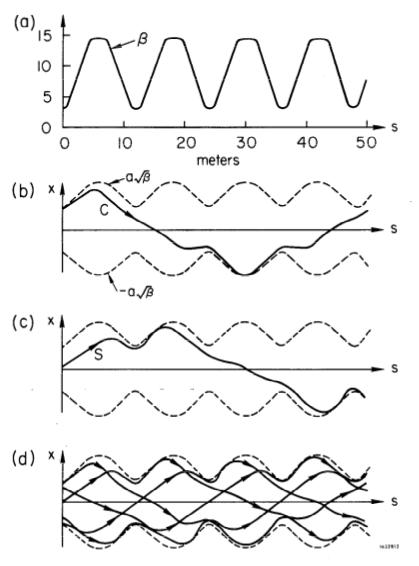
\includegraphics[width=0.7\linewidth]{./Figuras/fig12.jpeg}
	\caption{a) Betatron function. (b) Cosine-like trajectory for $s=O$. (c) Sine-like trajectory for $s=O$. (d) One trajectory on several successive revolutions.}
	\label{fig:fig12}
\end{figure}

One important feature of the betatron motion is evident in Fig.~\ref{fig:fig12}(d) -- at each physical azimuth the displacement $x$ of a circulating electron lies always below a limiting extreme value $X(s)$ obtained by setting $cos(\varphi - \vartheta) = 1$; namely
\begin{align}
	X(s) = a\sqrt{\beta(s)}
\end{align}
The complete trajectory of a stored electron will fall forever within an envelope defined by $\pm X(s)$. And it follows that the aperture required to contain an electron with a given oscillation amplitude varies around the ring as $X(s)$. The ratio of the envelope width at two locations $s_1$ and $s_2$ is, of course, just
\begin{align}
	\frac{X_2}{X_1} = \sqrt{\frac{\beta_2}{\beta_1}}
\end{align}
At each physical azimuth a stored electron may generally be expected to pass frequently with a displacement near the maximum.

Let's look now at the slope of the betatron trajectory, $x' = dx/ds$. Taking the derivative of Eq.~\eqref{eq:2.46}, we may write
\begin{align}
	x' = - \frac{a}{\sqrt{\beta}}\sin(\varphi-\vartheta)+\frac{\beta'}{2\beta}x\label{eq:2.52}
\end{align}
The first term comes from the changing phase; and the second from the variation of $\beta$.

Notice that the zeros of $x'$ -- and therefore, the peak values of $x$ -- do not occur when $cos(\varphi - \vartheta)$ is 1. Rather they are reached when
\begin{align}
	\tan(\varphi-\vartheta) = \frac{\beta'}{2}
\end{align}
which means that
\begin{align}
	\cos(\varphi-\vartheta) = \left[1+\frac{\beta'^2}{4}\right]^{-\frac{1}{2}}
\end{align}
If the peak of a particular cycle of an oscillation occurs at some $s$, the peak displacement then will be
\begin{align}
	x_{peak} = a\sqrt{\beta}\left[1+\frac{\beta'^2}{4}\right]^{-\frac{1}{2}}
\end{align}
See Fig.~\ref{fig:fig13}

\begin{figure}[!htb]
	\centering
	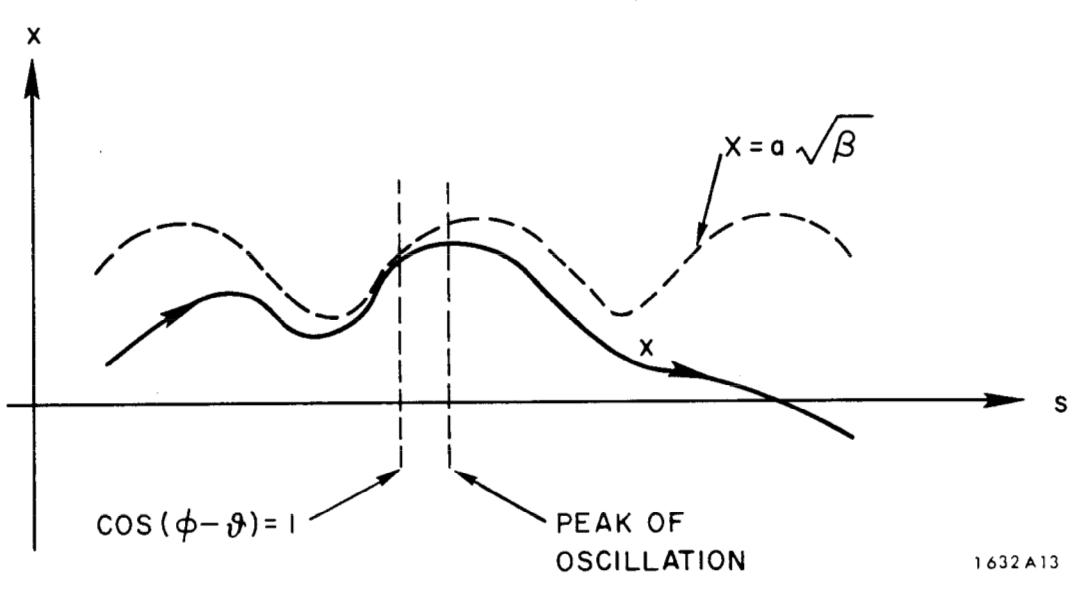
\includegraphics[width=0.8\linewidth]{./Figuras/fig13.jpeg}
	\caption{The maximum of a particular cycle of a betatron oscillation.}
	\label{fig:fig13}
\end{figure}

In a classical harmonic oscillation the amplitude is an invariant of the motion. Its square is proportional to the energy of the oscillator, and can be expressed as a quadratic function of the instantaneous position and velocity. The corresponding invariant of the pseudo-harmonic oscillator is the constant $a$.

If we isolate the cosine and sine terms in Eqs. \eqref{eq:2.46} and \eqref{eq:2.52}, square them, and add, we can relate $a^2$ to $x$ and $x'$. We find that
\begin{align}
	a^2 = \frac{x^2}{\beta} + \beta\left[x'-\frac{\beta'}{2\beta}x\right]^2\label{eq:2.56}
\end{align}
If we know $x$ and $x'$ at any azimuth, say $s_1$, $a$ can be found and all subsequent displacements can be expressed by
\begin{align}
	x = \frac{1}{\sqrt{\beta_1}}\left[x_1^2+\left(\beta_1x'_1-\frac{x_1\beta'_1}{2}\right)^2\right]^\frac{1}{2}\sqrt{\beta}\ \cos(\varphi-\vartheta)\label{eq:2.57}
\end{align}
The phase constant $\vartheta$ must also be determined from $x$ and $x'$. It can be obtained from
\begin{align}
	\tan(\varphi_1 - \vartheta) = -\frac{\beta_1 x'_1}{x_1}+\frac{\beta'_1}{2}
\end{align}
where $\varphi_1 = \varphi(s_1)$.

We are often interested only in the maximum value $X(s)$ which can be reached at any physical azimuth on any subsequent revolution. This maximum is independent of $\vartheta$ and is obtained by replacing the cosine factor of Eq.~\eqref{eq:2.57} by 1:
\begin{align}
	X(s) = \frac{1}{\sqrt{\beta_1}}\left[x_1^2+\left(\beta_1x'_1-\frac{x_1\beta'_1}{2}\right)^2\right]^\frac{1}{2}\sqrt{\beta(s)}
\end{align}

If $\beta$ were everywhere comparable -- say not too far from some typical value $\beta_n$ then the ensuing peak amplitude which would result from a sudden lateral displacement $\delta x$ would be about equal to $\delta x$, and the amplitude which would result from a sudden lateral impulse that changed the slope by $\delta x'$ would be about proportional to $\beta_n \delta x'$. Generally, we may expect that the amplitudes which result from disturbances to the trajectory will be less the smaller is $\beta$. Indeed, we may consider that $1/\beta$ is a measure of the “strength” of the lateral focusing, and that small values of $\beta$ are generally desirable.
